\documentclass[12pt,a4paper]{article}
\usepackage[latin1]{inputenc}
\usepackage{amsmath}
\usepackage{amsfonts}
\usepackage{amssymb}
\usepackage{graphicx}
\usepackage{scrlayer-scrpage}
\usepackage[xcdraw]{xcolor}
\usepackage{placeins}
\usepackage{slashbox}
\usepackage{colortbl}
\usepackage{pdfpages}
\usepackage[colorlinks, citecolor=red, linkcolor=blue]{hyperref}
\usepackage{geometry}
\geometry{right=25mm, left=25mm}
\usepackage{caption}
\usepackage{subfigure}
\usepackage{multirow}

%\usepackage{natbib}

\bibliographystyle{apalike}

%\setcounter{section}{-1}
\arrayrulewidth=1pt

\pagestyle{scrheadings}
\clearpairofpagestyles

\ihead{Andreas Mast}
\chead{Support Bracket Analysis}
\ohead{
\includegraphics[width=2cm]{Bilder/logo.jpg}}
%\ifoot{Fu�zeile innen}
\cfoot[\pagemark]{\pagemark}
%\ofoot{Fu�zeile au�en}

\renewcommand{\baselinestretch}{1.5}


%%%%%%%%%%%%%%%%%%%%%%%%%%%%%%%%%%%%%%%%%%%%%%%%%%%%%%%%%%%%%%%%%%%%%%%
% --Discussion anpassen, Wasserverlust und Kebabwechsel beim Ofen
% --Lineare Anpassung statt Logarithmischer Anpassung
%%%%%%%%%%%%%%%%%%%%%%%%%%%%%%%%%%%%%%%%%%%%%%%%%%%%%%%%%%%%%%%%%%%%%%%



%%%%%
% Start of the document
%%%%%

\begin{document}
	\pagenumbering{Roman}
	
	\begin{titlepage}
		\begin{center}
			
\includegraphics[scale=0.3]{Bilder/logo.jpg}
		\end{center}
		\vspace{1cm}
		\begin{center}
			{\huge Faculty of Computing, Engineering \& Science}	
		\end{center}
		\begin{center}
			{\Large Support Bracket Analysis}
		\end{center}
		\begin{figure}[h]
			\begin{center}
				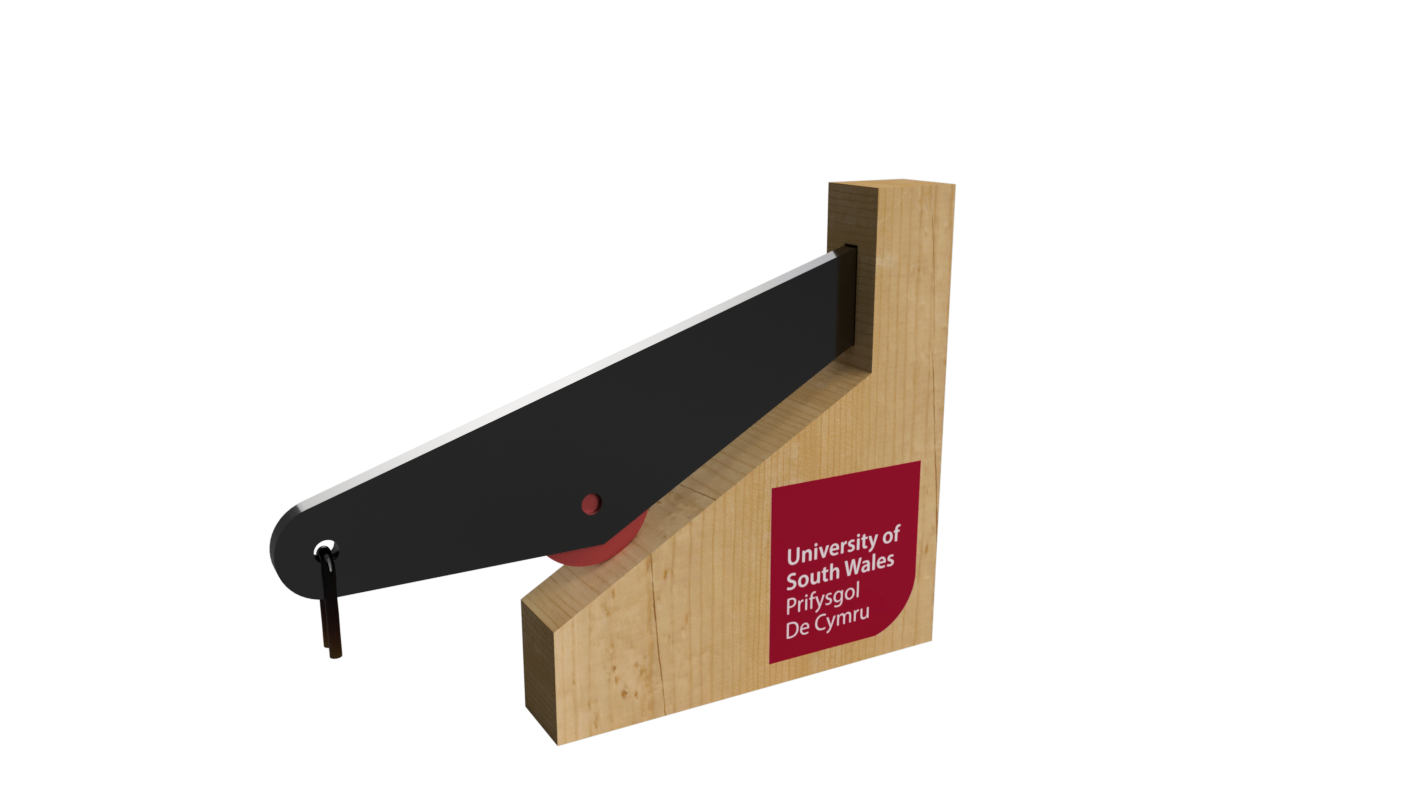
\includegraphics[scale=0.3]{Bilder/FEA_schema.png}
			\end{center}
		\end{figure}
		\begin{center}
			{\Large \today}
		\end{center}
%		\vspace{1cm}
		\begin{center}
%			\includegraphics[scale=0.7]{Bilder/Oven.png}
		\end{center}
%		\begin{center}
%			{\huge $4^{th}$ March 2018}			
%		\end{center}
%		\vspace{1cm}
		\begin{center}
			\begin{large}
				Andreas Mast - 17158885 
				
				mastandr@hs-albsig.de
			\end{large}
		\end{center}

	\end{titlepage}
	
	\newpage
	\pagenumbering{gobble}
	\tableofcontents
	\newpage
	\listoffigures
	\newpage
	\listoftables
	
	\newpage
	\pagenumbering{gobble}
	
	\pagenumbering{arabic}
 	
 	%%% mention of used software
 	
 	
	\section{Introduction}
	%General Introduction
	Support brackets are omnipresent and decisive for many construction, even if many people are not aware of them. As the name implies they support crucial parts of constructions by holding a weight or by holding two parts together. 
	
	%Problem description
	\subsection{Problem description}
	In this paper a support bracket with a specific load is investigated. For a better understanding of the assignment two oblique view of the given problem are shown in figure \ref{fig:schema}. Point A is fixed in all degrees of freedom and can not move anywhere. Point B is stabilized with a castor so that the bracket can not move in perpendicular direction to the diagonal wall. In Point C a load is applied. This load pulls the whole bracket downwards, which should be prevented through the wall.
	
	\begin{figure}[h]
		\subfigure[rendered oblique view]{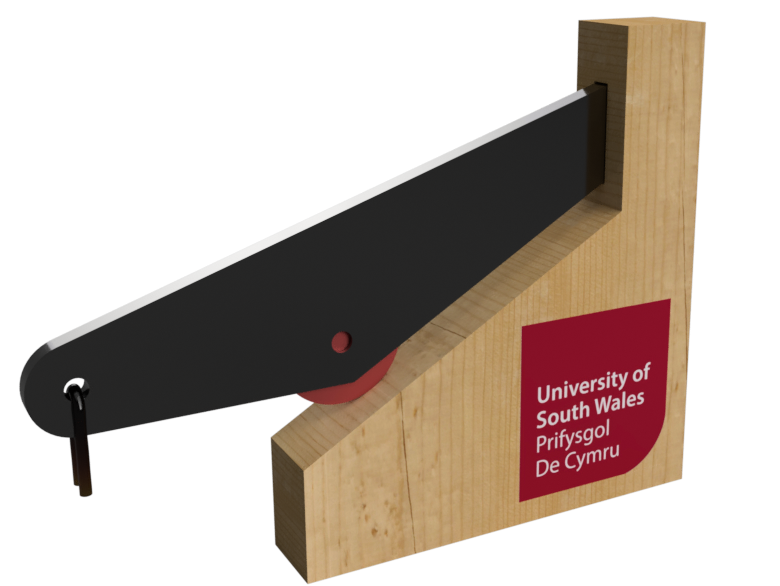
\includegraphics[height=6cm]{Bilder/FEA_schema_3.png}\label{test}}
		\subfigure[transparent oblique view]{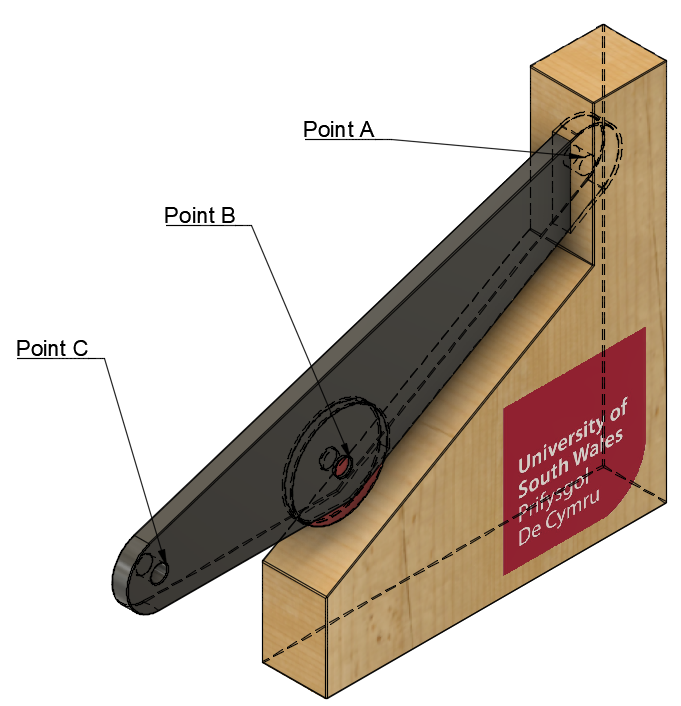
\includegraphics[height=6cm]{Bilder/FEA_schema_1.png}}
	
	\caption{Schematic representation of the given assignment}
	\label{fig:schema}
	\end{figure}

	\subsection{Given values}
	%Given Values
	For a better overview of the given assignment values, they are recorded in the following figure \ref{fig:problem_data} and table \ref{tab:given_values}. These values are approximations and necessary to analyse this problem. 

	\begin{figure}[h]
		\begin{center}
			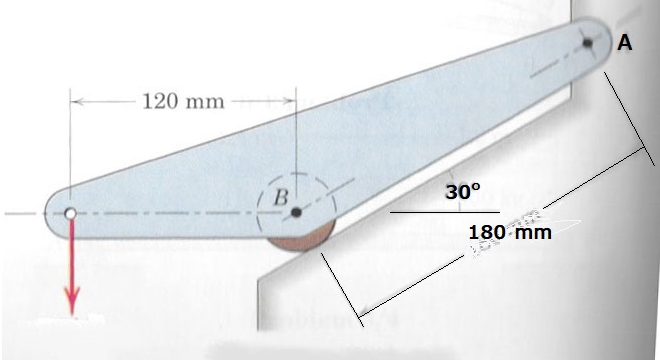
\includegraphics[scale=0.75]{Input/Exercise_Schema.png}
		\end{center}
		\caption{Front view of the given assignment}
		\label{fig:problem_data}
	\end{figure}
	
	\begin{table}[h]
		\begin{tabular}{|c|c|c|c|}
			\hline 
			Symbol & Description & Value & SI-Unit \\ 
			\hline 
			F & Applied Load & 1885 & $N = \frac{kg*m}{s^2}$ \\ 
			\hline 
			\multirow{2}{*}{} E &  Modulus of elasticity (aluminium 2014) & {$73 * 10^9$} &  $Pa =  \frac{N}{m^2} = \frac{kg}{m*s^2}$\\
			  				& \cite{matweb2018} &  & \\
			\hline 
			$\nu$ & Poisson's ratio & 0.33 & - \\ 
			\hline 
			thk & Bracket thickness & 10 & mm \\ 
			\hline 
		\end{tabular} 
	\caption{Given values from the assignment}
	\label{tab:given_values}
	\end{table}	
	
	
	%Basic of this Analysis
	\subsection{Objective of this analysis}
	The intention of this research is to determine, whether this support bracket can be used without any doubt of breaking under the given circumstances. To reach this goal it is fundamental to evaluate the internal stresses of this bracket and judge, whether a plastic deformation or even a rupture is likely to happen.
	
	\newpage
	
	
	\section{Assumptions}
	A realistic problem has an endless amount of variables influencing the results. This causes various problems. On the one hand it's possible to reach nearly a perfect analysis by including as much variables as possible. On the other hand imaginable to simplify an analysis by using some assumption, so that not every variable has to be taken into account.
	For this study the second approach is used. Therefore in the following some assumptions are made:
	\begin{enumerate}
		\item static
		\item homogeneous material
		\item isotropic material
		\item Linear elastic
		\item two dimensional
		\item plane stress (small thickness)
		\item weight can be ignored (no gravity)
		\item Evenly distributed load (1885 N at each point)
		\item Friction is ignored
		\item Axle/Pins are rigid
		\item Pins/Axle fits perfectly in holes
	\end{enumerate}

	\section{Modelling the analysis}
	
	\section{Results}
	
	\section{Discussion}
	
	\section{Conclusion}
	
	\newpage
	\bibliography{bib}
\end{document}


